\documentclass[13pt]{article}
\usepackage{amsmath}
\usepackage{amssymb}
\usepackage{amsthm}
\usepackage{color}
\usepackage{graphicx}
\linespread{1.7}
\title{A phylogenetic and population genetic model of amino acid substitution}
\author{}
\begin{document}
\maketitle
%%%%%%%%%%%%%%%%%%%%%%%%%%%%%%%%%%%%%%%%%%%%%%%%%%%%%%%%
\section{Abstract}
A new mechanistic model for the evolution of amino acid sequences is developed for studying the biological properties of proteins as well as phylogenetic estimation.  Two steps are bridged together to form a Markov process to describe substitutions between amino acids: mutation is based on general time reversible models for underlying nucleotides; fixation is obtained using classical population genetics theory. Selective restraints at amino acid level are characterized by the physiochemical distances between amino acids and the Grantham sensitivity coefficient exerted on the distances. Analysis of a yeast data set shows that the new model provides a better fit to data than the empirical models and reveals the variance of Grantham sensitivities and optimal amino acids at different sites in proteins.\\

\section{Introduction}
Importance of building accurate model for protein evolution. \\

Known models of amino acid replacement can be divided into two categories: empirical models and mechanistic models. Models in the first category include Dayhoff, JTT, WAG, LG, etc. Yang et al. (1998) implemented a few mechanistic models at the level of codons and explicitly modeled the biological processes involved, including different mutation rates between nucleotides, translation of the codon triplet into an amino acid, and the acceptance or rejection of the amino acid due to selective pressure on the protein. \\

Mechanistic models for the evolution of protein-encoding sequences are on three levels: mono-nucleotide level in DNA sequences, codon level in DNA coding sequences and amino acid level in protein sequences. Models on the DNA level use the most information and are more powerful to distinguish closely related sequences such as those caused by synonymous substitutions which are invisible at amino acid level. On the amino acid level, models can filter out some stochastic noise through the translation of DNA triplets to amino acids. Goldman and Yang (1994, MBE) constructed a codon-based model that uses the nucleotide-level information in DNA sequences and the amino-acid level information of synonymous and non synonymous nucleotide substitutions simultaneously. Their model incorporated transition / transversion bias, synonymous / nonsynonymous variation in a gene, and amino acid differences. The selective restraints at the amino acid level was accounted for by multiplying the substitution rate by a factor $\exp (d_{aa_i,aa_j}/V)$ where $d_{aa_i, aa_j}$ is the distance between amino acids $aa_i$ and $aa_j$ given by Grantham (1974) and $V$ is a parameter representing the variability of the gene or its tendency to undergo non synonymous substitution.\\

In Goldman and Yang's model, the Markov process is time reversible. In other words, the amino acids are equally as good in a protein and the substitution rates are  only proportional to the frequencies of the amino acids. However, from population genetics, the selective restraints should be a function of the fitness of proteins. Proteins with higher fitnesses get fixed with higher probability than those with low fitnesses. Gilchrist (2007) showed that the fitness of a protein is a function of factors including protein production cost, gene expression level, and functionality of protein. A protein might have a sequence of ``optimal" amino acids which give the protein best functionality, while other amino acids might also make the protein function but less well. Therefore, the functionality of a protein depends on what the optimal amino acids are and how far away the observed amino acids are from the optimal ones, as well as how sensitive the functionality is to the distance between amino acids. \\

In addition, the measure of difference between amino acids combines physiochemical properties that correlate best with protein residue substitution frequencies: composition, polarity and molecular volume. Grantham (1974) assigned weights to these three factors based on the average chemical distance given by the corresponding property alone. Take the composition for example, given the values for this property $c_i$'s, the weight $\alpha = (1/\bar{D}_c)^2 = 1.833$ where $\bar{D}_c = \sum[(c_i - c_j)^2]^{1/2}/190$. Similarly the weights for polarity and molecular volume are $0.1018$ and $0.000399$. Since the values for the volume property is much bigger than the other 2 properties its weight is much smaller. We call the weights Grantham weights. It is reasonable to believe that in some genes one property might play a more important role while in some genes it might be another property. For example ?  We present a new model that incorporates the above factors by including the Grantham weights $\alpha, \beta, \gamma$ and the sensitivity of functionality to distance from the optimal amino acid as parameters. We call the sensitivity coefficient ``Grantham sensitivity'' and denote is by $g$.\\

In this paper we characterize our amino acid-based model, which incorporates substitution rates of underlying coding nucleotides, the biological properties of amino acids, selection sensitivity of amino acid differences. We use the model for maximum likelihood (m.l.) estimation of phylogenies and apply the model to Rokas's yeast data sets with 8 species. The results are compared with those under previous amino-acid models. We also investigate the evolution process of protein with different parameters.\\
(and use simulations and information from empirical data to find cases where populations of intermediate size may evolve faster than populations of large size.)

%%%%%%%%%%%%%%%%%%%%%%%%%%%%%%%%%%%%%%%%%%%%%%%%%%%%%%%%
\section{Model}
Our model works for homologous protein-coding sequence without gaps or with gaps removed. We use a continuous time Markov process to model substitutions among the amino acids within a protein coding sequence. The states of the Markov process are the 20 natural amino acids (nonnatural amino acids can be easily added), so we use a $20 \times 20$ rate matrix $Q=(Q_{ij})$ where $Q_{ij}$ represents the instantaneous rate that amino acid $i$ will be substituted by amino acid $j$. The rate matrix $Q$ is obtained by multiplying the mutation rate matrix $M$ and fixation probability matrix $F$. As usual the row sum of $(Q_{ij})$ equals $0$ and $P(t) = \exp (tQ)$, where $P_{ij}(t)$ is the probability that amino acid $j$ replaces $i$ after time $t$.\\

\subsection{Methods}
For all time reversible models, the substitution rate matrix is a product of a symmetric matrix $S$ and the the base frequencies of different states: $Q = S\Pi$, where $S$ is called the exchange rate matrix and $\Pi$ is a diagonal matrix of the base frequencies. The mutation rate matrix for 20 amino acids are derived from the $4 \times 4 $ exchange rate matrix for nucleotides. This reduces the number of rate parameters from 190 to 6 comparing to treating all the amino acid exchange rates as parameters.\\

We assume that mutations occur independently between nucleotides at the same codon position. Therefore, mutations involving more than one position during time $\Delta t$ will have probabilities on the order of $\Delta t^2$ and are, therefore, ignored. First, a $61 \times 61$ sense codon exchange rate matrix is obtained. The rate between codon $i$ and $j$ is equal to the rate between the pair of nucleotides if that is the only different pair in all 3 codon positions, and 0 otherwise.\\


Second, using the genetic code table, we group the codons that coding for the same amino acid to get the $20 \times 20$ exchange rate matrix $S$ for all amino acids. Suppose the sets of codons for amino acids $i$ and $j$ are $I$ and $J$ correspondingly, i.e. $aa_u = i$ for $u \in I$, and $aa_v = j$ for $v \in J$. Combining synonymous codons that code for amino acid $j$ into one state, we have $\pi_J = \sum_{v \in J} \pi_v$ as the equilibrium frequency of amino acid $j$. The exchange rate matrix for a reversible Markov process of amino acid mutation $S$ has entries:
\[\mu_{IJ} = \sum_{u \in I} \sum_{v \in J} \pi_u \pi_v s_{uv} / (\pi_I \pi_J)\]
\noindent
And $q_{IJ} = s_{IJ} \pi_J$ with $s_{IJ}  = s_{JI}$ constitutes the mutation rate matrix $M$. For detailed derivation see Yang(MBE 1998). The mutation process is time reversible, i.e. $\pi_I \mu_{IJ} = \pi_J M_{JI}$ is satisfied for all $1 \le I,J \le 20$. We assume that for each amino acid its different genetic codes have the same frequency. Therefore, the mutation rates between amino acids only depend on the frequencies of amino acids. \\

Studies show that fixation of mutations between dissimilar amino acids is generally rare. Therefore, in addition to the effects of mutation bias our model also considers the effects of natural selection on the amino acid sequence of a gene. We begin by assuming that there is an optimal amino acid for each position in a protein and non-optimal amino acids are subjected to natural selection. The functionality of an amino acid depends on the scaled physiochemical distance (Grantham, Science 1974) between the observed and optimal amino acids, the sensitivity of the protein's function to the physicochemical distance and the protein production rate of the gene. \\

%%%intro of the physicochemical distance between amino acids, from Grantham's paper%%%
Among the properties of amino acid side chain that correlate with relative substitution rate, composition ($c$), polarity ($p$) and molecular volume ($v$) have strongest correlation. Composition is defined as the atomic weight ratio of noncarbon elements in end groups or rings to carbons in the side chain. The last two properties are from published data (add ref). The overall physicochemical difference between any two amino acids $i$ and $j$ combines the three properties: $d_{ij} = [\alpha (c_i-c_j)^2 + \beta (p_i - p_j)^2 + \gamma (v_i - v_j)^2]$ where $\alpha, \beta, \gamma$ are the corresponding weights for the 3 components. Grantham weighted the 3 components by dividing them by the mean distance found with that property alone in the formula. The values of the weights found this way are $\alpha = 1.833$, $\beta = 0.1018$, $\gamma = 0.000399$. These weights are used for amino acids in all genes of any species. However, depending on the functions and environment of amino acids, it is reasonable to assume that the impact of different properties varies. In our model, the weights $\alpha, \beta, \gamma$ are treated as estimable parameters rather than being fixed. The distances are scaled so that the mean pairwise distance is 1. Because of the scaling, only 2 of the 3 weights are free parameters. We fix the weight $\alpha$ to be $1.833$ as in Grantham's weights, and estimate $\beta, \gamma$. \\

Suppose a protein of length $n$ has the optimal amino acid sequence $\hat{\mathbf{a}} = (\hat{a}_1, \hat{a}_2, \cdots \hat{a}_n)$, the observed sequence of amino acids is $\mathbf{a} = (a_1, a_2, \cdots, a_n)$, the Grantham sensitivity coefficient vector is  $\mathbf{g}=(g_1,g_2,\cdots,g_n)$.
The distance vector $\mathbf{d} = (d_1, d_2, \cdots, d_n)$ represents the distance per amino acid basis from the optimal. The functionality of a protein $\mathbf{a}$ with $n$ amino acids is then defined as

\begin{equation}
F(\mathbf{a}| \hat{\mathbf{a}},\mathbf{g})  =  \frac{n}{\displaystyle  \sum_{k=1}^n{(1+d_kg_k)}} \label{eq:harmonic}\\
\end{equation}
In order to simplify notation, the parameters $\hat{\mathbf{a}}$ and $\mathbf{g}$ will be omitted from now on if there is no potential confusion.\\

%functionality to fitness%
As in Gilchrist 2007, the fitness of a protein is related to its functionality in the following way:
\[f(\mathbf{a}) \propto \exp\{-\frac{C\Phi q}{F(\mathbf{a})}\}\]
where $C$ is the expected cost of producing a single complete protein, $q$ is a scaling constant (seconds per ATP) determining the relationship between the rate of ATP usage and fitness $f$, and $\Phi$ is a measure of gene expression, specifically protein production rate for a given gene.
Combining $C\Phi q$ as one constant $A$, we have
$f(\mathbf{a}) \propto \exp\{-\frac{A}{F(\mathbf{a})}\}$.
Clearly, protein fitness is an increasing function of functionality.\\

%fixation probability 
Following Sella-Hirsh (Add reference), if there is a single mutant $\mathbf{a}_j$ from a diploid population of effective size $N_e$ with wild type $\mathbf{a}_i$, the probability of the mutant getting fixed in the population is 
\begin{equation}
\pi_{ij} = \pi(\mathbf{a}_i \rightarrow \mathbf{a}_j ) = \frac{1-f(\mathbf{a}_i)/f(\mathbf{a}_j)}{1-(f(\mathbf{a}_i)/f(\mathbf{a}_j))^{2N_e}}
\label{eq:fixation}
\end{equation}
where $f(\mathbf{a}_i)$ and $f(\mathbf{a}_j)$ are the fitnesses of genotypes $\mathbf{a}_i$ and $\mathbf{a}_j$. This formula is valid under the condition $s, \frac{1}{N}, Ns^2 \ll 1$ where $s$ is the selelction advantage/disadvantage of the mutant over the wild type. (Add ref or delete)\\

%It is an approximation to the canonical formula 
%
%\begin{equation}
%\pi(\mathbf{a}_i \rightarrow \mathbf{a}_j,p) = \frac{1-e^{-2N_e ps}}{1-e^{-2N_es}}
%\label{eq:fixcanonical}
%\end{equation}
%
%\noindent where $p$ is the initial frequency of the mutant, and $s=(f_j-f_i)/f_i$ is the selection advantage of $\mathbf{a}_j$ comparing to $\mathbf{a}_i$ (note here $s$  is different from the selection strength defined above on the distance from optimal protein).
%When there is a single mutant in the population, i.e. $p=1/(2N_e)$, the formula simplifies to 
%$(1-e^{-s})/(1-e^{-2N_es})$. Both S-H and the canonical formulae are valid under the same condition: $s, \frac{1}{N}, Ns^2 \ll 1$.\\




In the S-H formula of the fixation probability, the determining value is $f_i/f_j$.
Based on the definition of functionality in Equation \ref{eq:harmonic}, we have the following:

\begin{equation}
\frac{f(\mathbf{a}_i)}{f(\mathbf{a}_j)} = \prod_{k=1}^n\Big( \frac{f(\mathbf{a}_i^k)}{f(\mathbf{a}_j^k)}\Big)^{\frac{1}{n}}
\end{equation}


i.e. the fitness ratio of the two genotypes is the geometric mean of the fitness ratios between the two amino acids at all sites. Therefore, when $\mathbf{a}_i$ and $\mathbf{a}_j$ only differ at position $k$, this fitness ratio simplifies to  
\begin{eqnarray}
\frac{f(\mathbf{a}_i)}{f(\mathbf{a}_j)} & = & \Big( \frac{f(\mathbf{a}_i^k)}{f(\mathbf{a}_j^k)}\Big)^{\frac{1}{n}}\\
 & = &\exp \Big[-A\Big( \frac{1}{F(\mathbf{a}_i )} - \frac{1}{F(\mathbf{a}_j )}\Big)\Big] \nonumber\\
%& = & \exp\Big[ -\frac{A}{n}(d_k^i s_k - d_k^j s_k)\Big]\\
%& = & \exp\Big[ -\frac{C\Phi q}{n}(d_k^i s_k - d_k^j s_k)\Big]\\
& = & \exp\Big[ -\frac{C\Phi q g_k}{n}(d_k^{(i)} - d_k^{(j)})\Big] \label{eq: ratio}
\end{eqnarray}
\noindent
this quantity is only related to site $k$. From equation \ref{eq: ratio}, it is easy to see that all the sites are independent in the sense that if there are more than 1 site that differ, the ratio is simply a product of ratios at all sites. \\

For a single site, we have 
\begin{equation}
\frac{f(a_i)}{f(a_j)} = \exp\Big(-C\Phi q g(d^{(i)}-d^{(j)})\Big)
\label{eq: ratiosingle}
\end{equation}
%%%%%%%%%%%%%%%%%%%%%%%%%%%%%%%%%%%%%%%%%%%%%%%%%%%%%%%
%continue revision from here
%%%%%%%%%%%%%%%%%%%%%%%%%%%%%%%%%%%%%%%%%%%%%%%%%%%%%%%
From Equation \ref{eq:fixation} and \ref{eq: ratiosingle}, for a single mutant at one site of a protein in a diploid population of size $N_e$, the fixation probability of this mutant depends on the physicochemical distances $d$ from the optimal amino acid at this site, sensitivity coefficient $g$ of functionality to the distance $d$, and constants $C$, $\Phi$, $q$, $N_e$.\\


Therefore, the instantaneous substitution rate $q_{ij}$ from $\mathbf{a}_i$ to $\mathbf{a}_j$ is 2 times the product of effective population size $N_e$, mutation rate $\mu_{ij}$ from $a_i$ to $a_j$ and the fixation probability of a single mutant:
\begin{equation}
u_{ij} = 2N_e \mu_{ij} \pi_{ij}
\label{eq:subrate}
\end{equation}
Note that $\mu_{ij} = 0$ when more than 1 position differ in the genetic codes for $a_i$ and $a_j$ and that the mutation rate and fixation probability are both amino acid specific. \\

Given the values for $(M_{nu},g, \alpha, \beta, \gamma, C, \Phi, q, N_e)$, the frequencies of different amino acids and the optimal amino acid at a site, we can calculate the $20 \times 20$ instantaneous substitution rate matrix $Q$ for the Markov process. $Q$ is scaled by the frequencies of amino acids to satisfy $\sum_{i=1}^{20} \pi_i q_{ii}= -1$. Under this restraint, the length of a branch represents the expected number of substitutions on the branch. With the probabilities $P(t)  = \exp(Qt)$ the log-likelihood for a given tree topology can be calculated following Felsenstein (1981). Since all sites are independent, we can calculate the likelihood of observing the sequence data at the tips of a phylogenetic tree $T$ with given topology and branch lengths by multiplying the likelihood values at all sites.\\

%table of parameters in the model%
\begin{table}[h]
\centering
\caption{parameters in the model}
\begin{tabular}{ c p{6cm} }
\hline
$s_{ij}$ & exchange rates between nucleotides $i$ and $j$ \\
$g$       & sensitivity coefficient of functionality to physicochemical distance \\
$(\alpha,\beta,\gamma)$ & weights for the 3 physicochemical properties in amino acid distance formula \\
$C$ & cost of producing a protein\\
$\Phi$ & expression level \\
$q$ & scaling factor \\
$N_e$ & effective population size \\
\hline
\end{tabular}

\label{tb: para}
\end{table}

\subsection{Identification of optimal amino acids}
To calculate the likelihood values, the optimal amino acids need to be specified. We implement 3 approaches to identify the optimal amino acid at a certain site. First one is called ``max rule''. We calculate the likelihood values when each of 20 amino acids is optimal with all other parameters given and choose the one that maximizes the likelihood as optimal. This method treats the optimal amino acids as parameters to be estimated in the maximum likelihood computation. The number of parameters increases with the number of distinct sequence patterns at the tips, which often is a big number. \\
Second approach uses the ``majority rule'', i.e. the most frequent amino acid in the sequence is chosen as the optimal amino acid. If more than 1 amino acid has the same highest frequency, then one of them is picked randomly as optimal. If the sequences have evolved long enough to reach equilibrium, the optimal amino acid has the highest probability to be observed. If the evolving time is short, or there are not enough substitutions during evolution process, the optimal amino acids estimated this way can be inaccurate. \\
The third method is ``weighted rule''. 20 amino acids are assigned weights of being optimal. If the same weights are used for all sites, then the number of parameters added is 19 compared to hundreds or more in the first approach. The weights are expected to vary with the environment, function of proteins and other factors. Therefore an alternative is to use different weights for different genes or gene groups in a protein sequence. \\
It is apparent that the first method gives the best likelihood value but uses the most parameters. The third method uses a lot fewer parameters. However, if the optimal amino acids vary a lot between different sites, the maximum likelihood values will decrease significantly. We'll compare the performance of different approaches in the Results section.\\

\subsection{Identifiability of parameters}
Since $C, \Phi, q$ and $g$ are multiplied together as a composite parameter, we fix the values of $C, \Phi, q$ and search for MLE for $g$. As mentioned earlier, for the weights used in the Grantham distance formula, $\alpha$ is fixed and $\beta, \gamma$ are estimated.  In addition, the effective population size is assumed to be fixed in this paper. Suppose the phylogenetic topology is given, we are estimating the following parameters: $g, \beta/\alpha$, $\gamma/\alpha$, frequencies of amino acids, branch lengths, and the exchange rate matrix for nucleotides. 

\section{Results}
%\subsection{Model consistency}
%To assess the model accuracy, we first simulate data using different parameter values, find the MLEs for the parameters from the simulated data, and then investigate the accuracy of the estimates by looking at the mean squared error and confidence intervals.\\


\subsection{Results on Rokas et al.'s data on yeast}
We analyzed data previously studied by Rokas (2003 Nature). This genome sequence data have been obtained for 7 {\it Saccharomyces} species ({\it S. cerevisiae, S. paradoxus, S. mikatae, S. kudriavzevii, S. bayanus, S.castellii} and {\it S. kluyveri}) as well as for the outgroup fungus {\it Candida albicans}. It includes 106 genes that are distributed throughout the {\it S. cerevisiae} genome on all 16 chromomosomes and comprises a total length of 42,342 amino acids. We use the tree topology that is supported by the concatenated genome sequence.\\

\subsubsection{maximum likelihood estimation}
First, the 106 gene sequences are concatenated as 1 whole sequence with 42,342 amino acids. We use ProtTest to find maximum log likelihood values under empirical models and compare their AIC values. We also find the maximum log likelihood values under our new model, with all 3 approaches to treat the optimal amino acids. In all the analyses, tree branch lengths are optimized while topology is not. \\

The log likelihood values and the AIC values are compared in Table 2. Under the empirical models, the substitution rates are fixed instead of being optimized. $I$ denotes that proportion of invariable sites is estimated in the model, $G$ means that the model includes the rate variation as a Gamma distribution across all the sites. In models with $F$, amino acid frequencies are treated as free parameters and estimated by the observed frequencies in the sequence data. Otherwise, the amino acid frequencies are the equilibrium (stationary) frequencies under the substitution rate matrix.\\

Under the new model, amino acid frequencies are treated as 19 free parameters and estimated from the observed frequencies in the sequence data. In addition, 5 free parameters for exchange rates between nucleotides, 14 branch lengths for the 8-species phylogeney, Grantham sensitivity $g$, 2 free parameters for the weights in the physicochemical distance formula $\beta$ and $\gamma$ are optimized in the maximum likelihood analyses.\\


All the parameters are treated the same across all the sites except the optimal amino acids. The loglikelihood and AIC values are also compared with those under empirical models for amino acids from ProtTest (reference). \\

\begin{table}[h]
\begin{center}
\caption{Log-likelihood values and parameter estimates under empirical models and new model for the amino acid sequences of length 42,342}
\begin{tabular}{l c c c r}
\hline
Model & $\Delta$AIC & $l$ & Tree length & Parameters \\
\hline
New+maj & 0.00 & -273239.30 & & 41 \\
New+max & 11358.60 & -236576.60 & 12.39 & 42,383 \\
New+weights & 94363.00 & -320401.80 & & 60 \\
LG+I+G+F & 50905.58 & -298699.09 &  & 34\\
LG+G+F & 50910.46 & -298699.09 & & 33 \\
\hline
\end{tabular}
\end{center}

Note: The last two models in the table are the best models picked out by ProtTest.
\label{table:mle}
\end{table}

If the optimal amino acids are not counted as free parameters being estimated, the majority approach gives the best AIC value. $\Delta$AIC value for the best empirical model LG + I +G + F is about 50,000 units, which indicates a substantially better fit under the new model. One thing need to point out is that under the maximizing approach for identifying optimal amino acids at each position in the sequence, the number of parameters is much bigger. However, the improvement of log likelihood is so big that this model still performs much better than the best empirical model, with AIC value 40,000 units smaller. With the weighted approach, i.e. for each site, every amino acid has the same probability of being optimal, the increase in the log likelihood outweighs the saving in the number of parameters. This also indicates that the optimal amino acids at all sites vary a lot.  

\subsubsection{Parameter variation between genes}
We also analyzed Rokas et.al.'s data gene by gene. The best tree branch lengths  and the exchange rate matrix for the concatenated genomic sequence are used in the analysis. Grantham sensitivity and the weights in the physicochemical distance formula are optimized for each gene. Under both approaches of obtaining the optimal amino acids, the estimates for all 3 parameters are on the similar scale. As expected, the weights for physicochemical properties are also similar to the ones that Grantham used. Figure \ref{fig:correlation} showed the correlation between $\beta$ and $\gamma$. Linear regression suggests strong linear relationship between the 2 parameters, especially under the maximizing rule where $R^2$ is very close to 1.\\

Since the variation of Grantham weights is small, we fixed $\beta$ and $\gamma$ across all genes and optimized $g$ for each gene given the values of $\beta$ and $\gamma$ to get the maximum likelihood. We then did optimization on the common physicochemical weights $\beta$ and $\gamma$. The ML estimates are $\beta = 0.1244$ and $\beta = 0.0005917$, comparing to Grantham's weights $\beta = 0.1018$ and $\beta = 0.000399$.\\

Notice in Figure \ref{fig:betagamma} and \ref{fig:gvalue}  there is an outlier for the estimates of Grantham weights with the maximizing rule, which corresponds to gene 63; this also happens to gene 48 with estimates of sensitivity values. There are several possible explanations. One is discrepancy between the gene trees. We use the same tree (topology and branch lengths) for all the genes, however, sequences in some genes might support a different phylogeny. Another possibility is that these genes have very different structures from other genes so that the importance of the physicochemical properties is very different. (Look at the gene trees and see if they have different topologies from the one that is used in the ML analysis)\\


\begin{figure}[ht]
\caption{The figures in the first row are the estimates of $\beta$ and $\gamma$ using the maximizing rule, in the second row are the estimates of $\beta$ and $\gamma$ using the majority rule. Notice the difference in the range of y-axis}
\centering
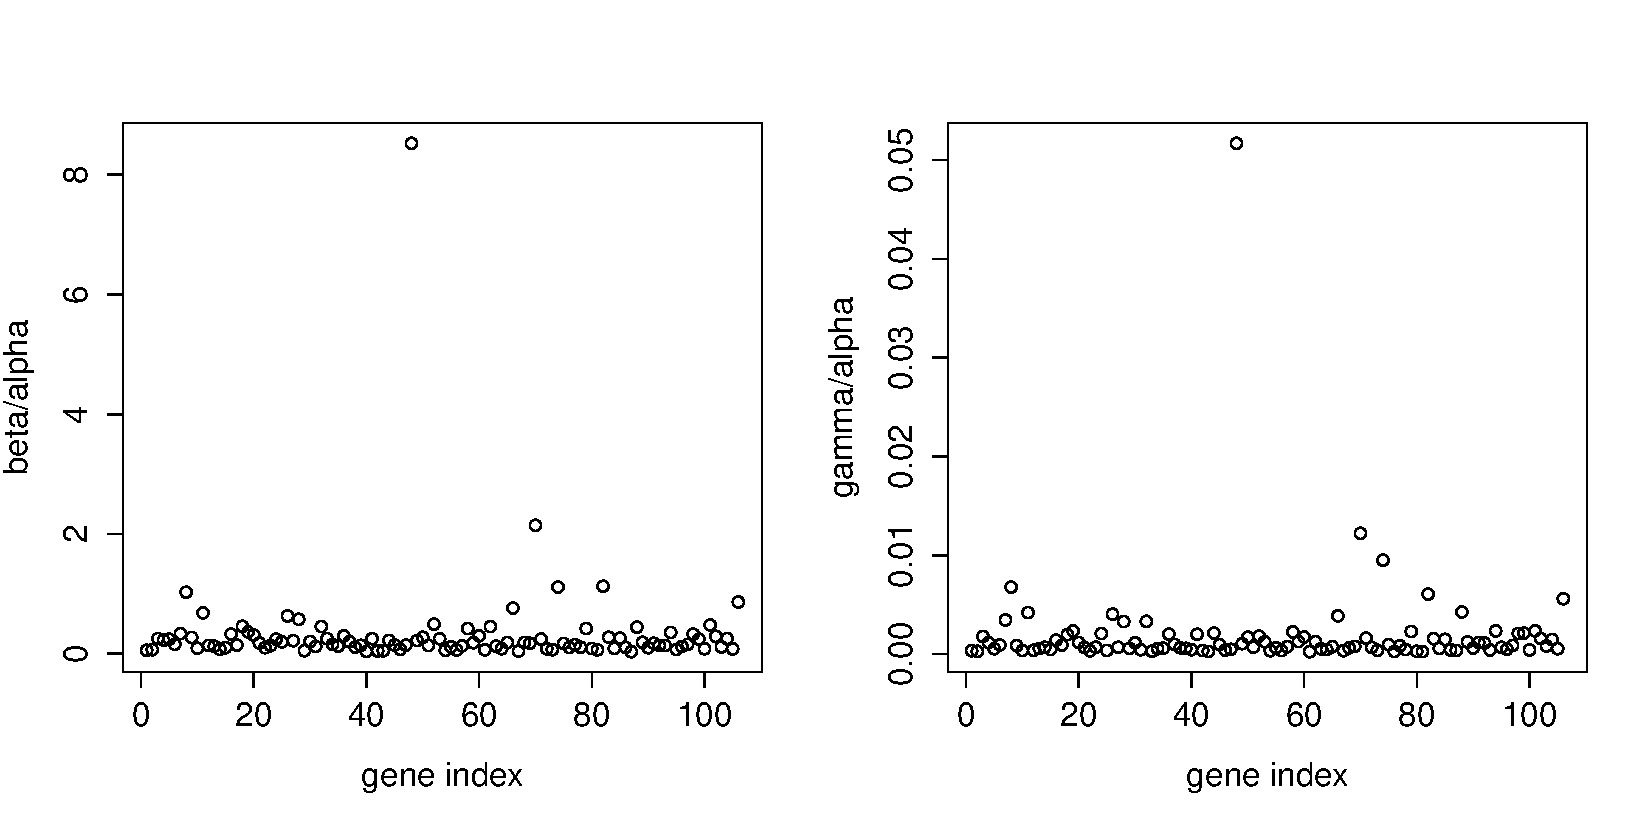
\includegraphics[width=\textwidth]{betagamma.pdf}
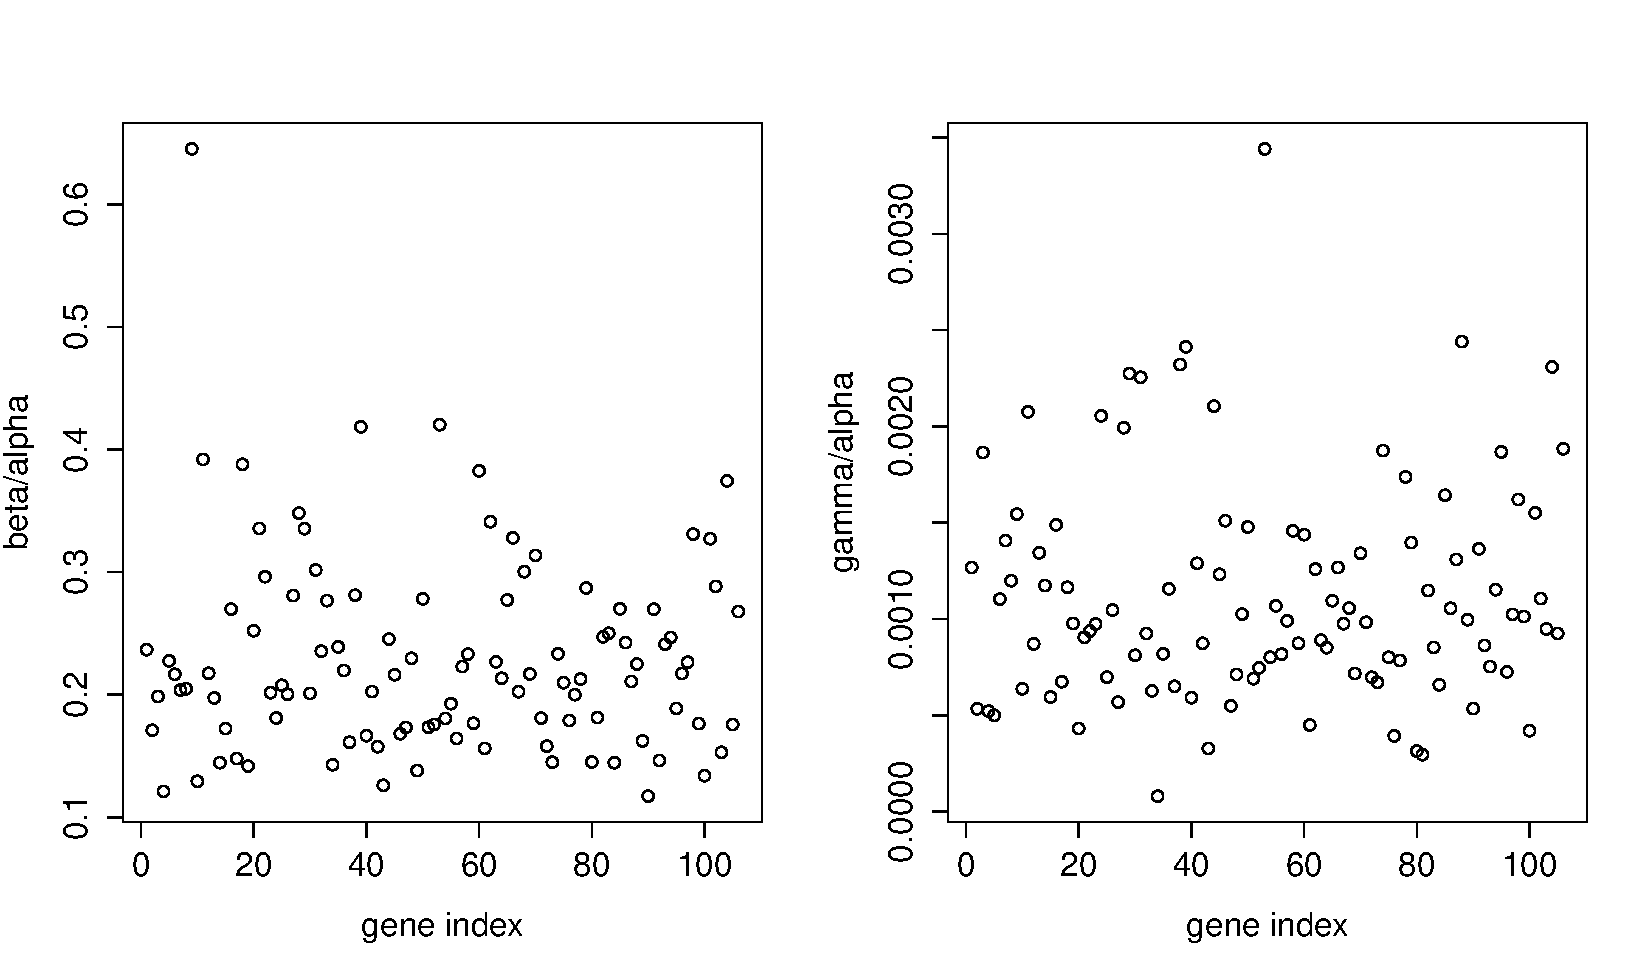
\includegraphics[width=\textwidth]{betagamma2.pdf}
\label{fig:betagamma}
\end{figure}

\begin{figure}
\caption{Correlation between $\beta$ and $\gamma$. Blue line is the maximizing rule, with $R^2 = 0.9899$, Red line is the majority rule with $R^2 = 0.3258$}
\centering
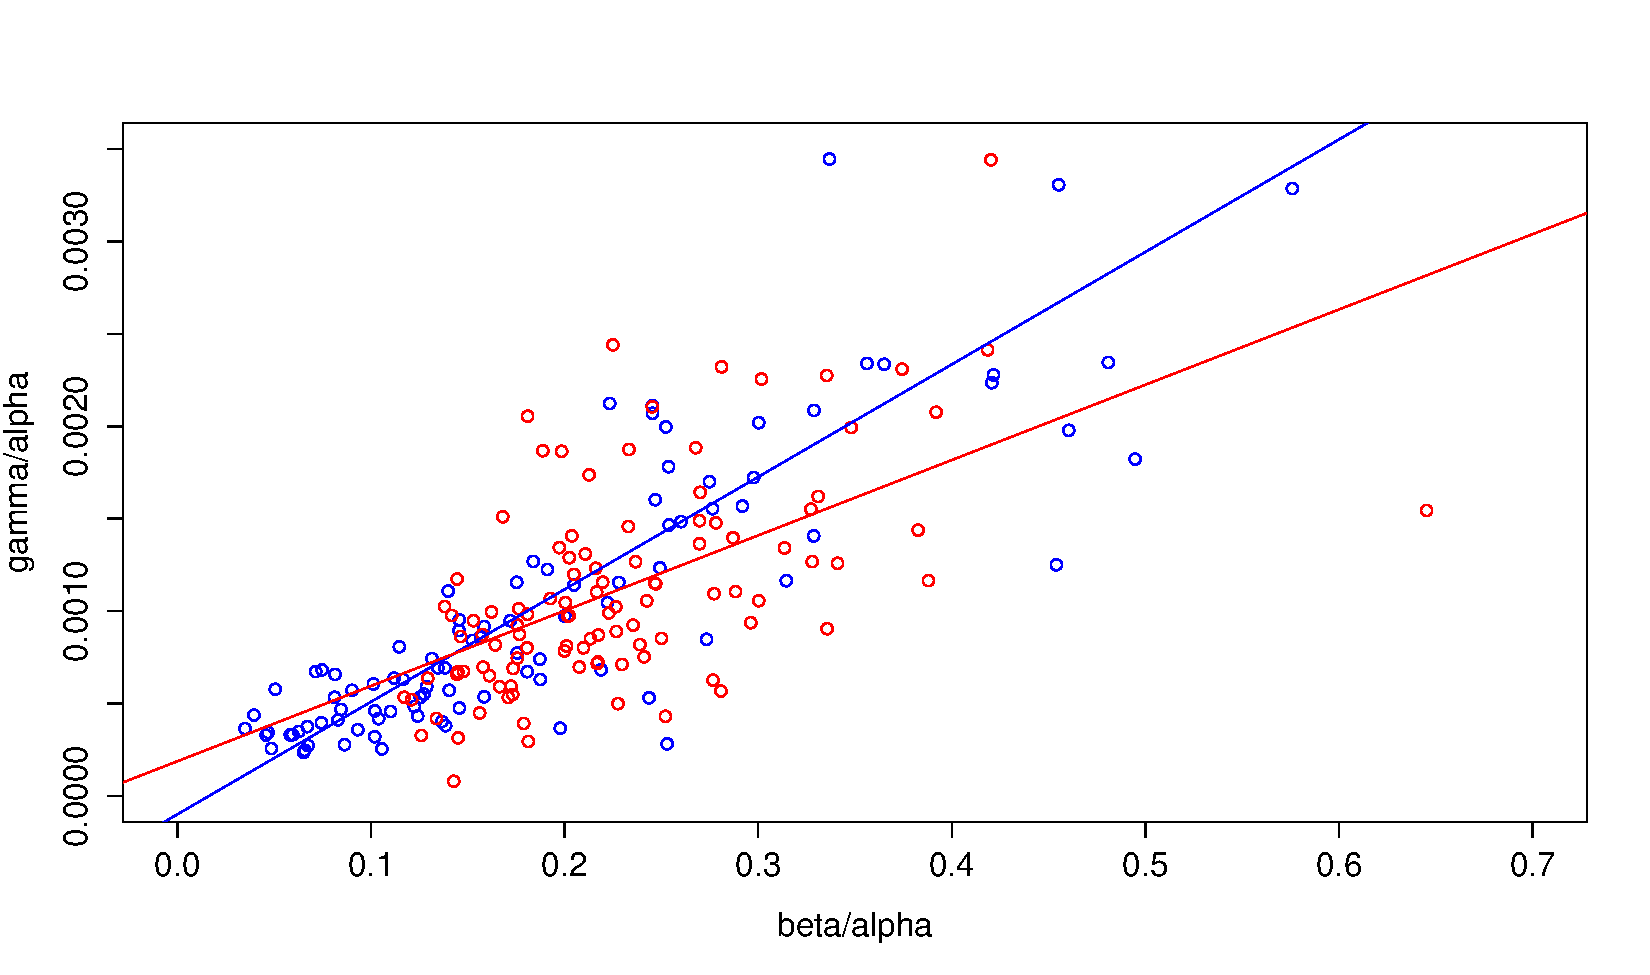
\includegraphics[width=\textwidth]{GMmaxmaj.pdf}
\label{fig:correlation}
\end{figure}

\begin{figure}[ht]
\caption{Plots of Grantham sensitivity across all the genes. On the left, optimal amino acids are obtained using maximizing rule; on the right majority rule}
\centering
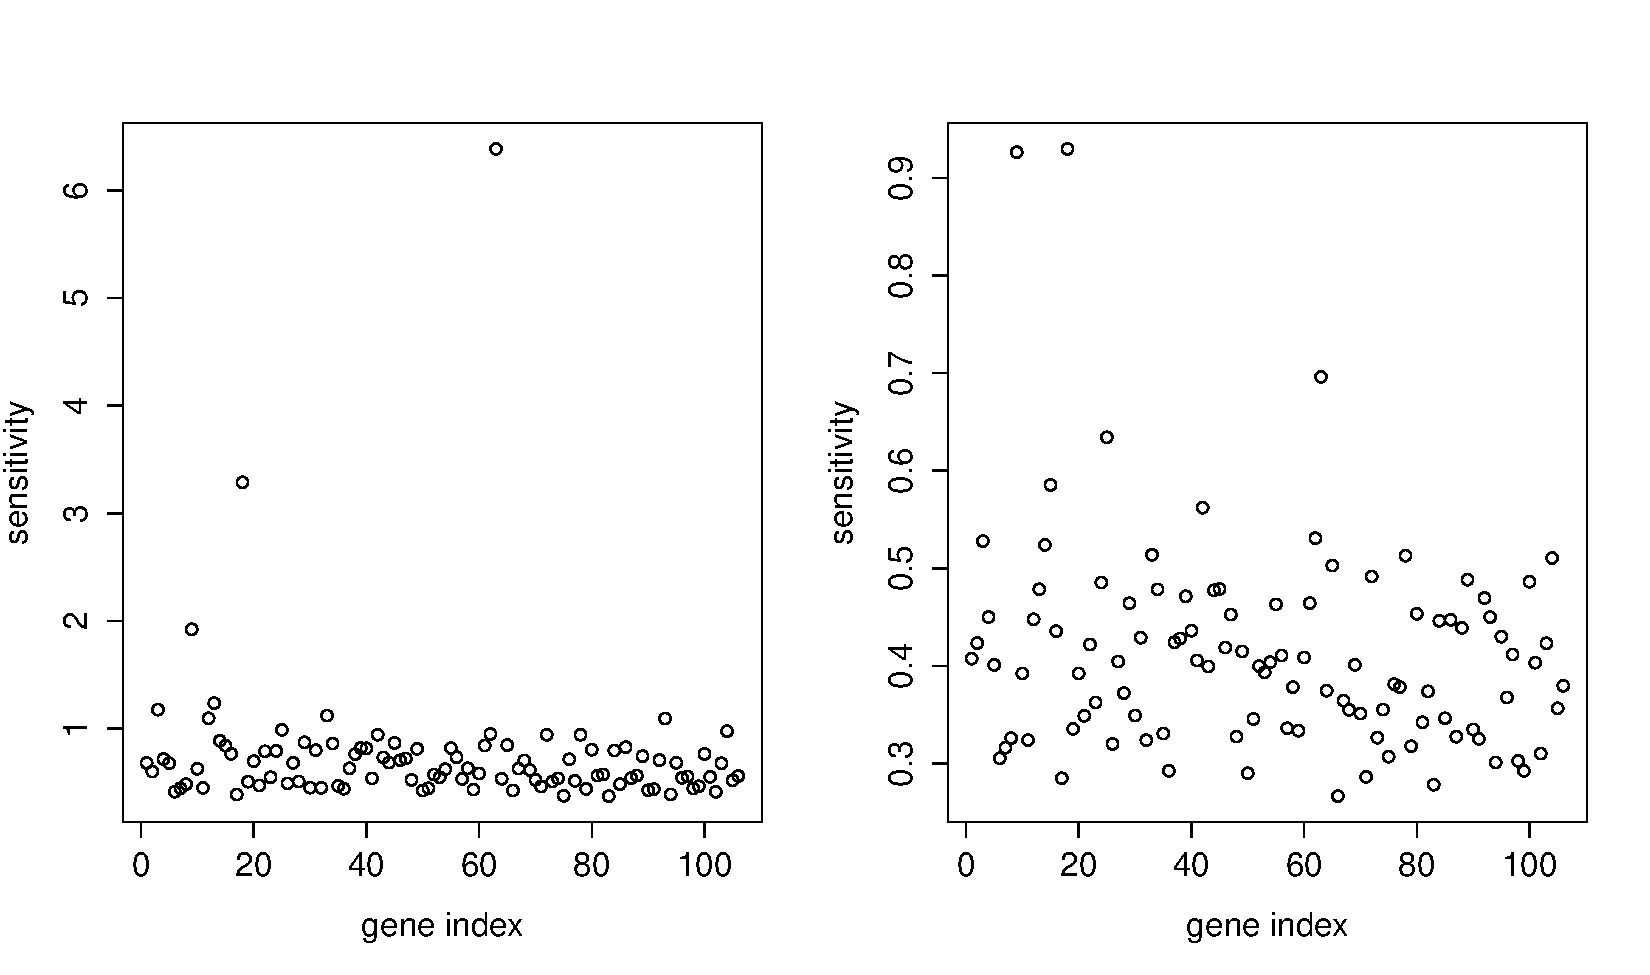
\includegraphics[width=\textwidth]{gvalue.pdf}
\label{fig:gvalue}
\end{figure}


\subsubsection{Model accuracy}
To assess model accuracy, we did simulations using the maximum likelihood estimates from Rokas et. al. 's data. (waiting on results)

\end{document}